\documentclass[11pt]{article}

% ---------------------------------------------------------
% Packages
% ---------------------------------------------------------
\usepackage[a4paper, margin=1in]{geometry}
\usepackage[utf8]{inputenc}
\usepackage{amsmath, amssymb, amsthm}
\usepackage{setspace}
\usepackage{graphicx}
\usepackage{float}
\usepackage{caption}
\usepackage{subcaption}
% Ensure floats are not placed inside code listings
\IfFileExists{placeins.sty}{\usepackage{placeins}}{}
\usepackage{booktabs}
\usepackage{hyperref}
% Load enumitem if available (some TeX installations may omit it)
\IfFileExists{enumitem.sty}{\usepackage{enumitem}}{}
\usepackage{mathtools}
% Load physics if available (not present in some minimal TeX installs)
\IfFileExists{physics.sty}{\usepackage{physics}}{}
\usepackage{bm}
\usepackage{listings}
\usepackage{xcolor}


% ---------------------------------------------------------
% Code block style
% ---------------------------------------------------------
\lstset{
    inputencoding=utf8,
    extendedchars=true,
    basicstyle=\ttfamily\small,
    keywordstyle=\color{blue},
    commentstyle=\color{gray},
    stringstyle=\color{orange},
    breaklines=true,
    columns=fullflexible
}

% ---------------------------------------------------------
% indentation
% ---------------------------------------------------------
\setlength{\parindent}{0pt}


% ---------------------------------------------------------
% Hyperlink setup
% ---------------------------------------------------------
\hypersetup{
    colorlinks=true,
    linkcolor=black,
    urlcolor=blue,
    citecolor=blue
}

% ---------------------------------------------------------
% Title
% ---------------------------------------------------------
\title{
    \vspace{-1cm}
    \textbf{Lab 1 Report}\\
    \vspace{0.2cm}
    Summer 2026
}
\author{
    Soeun Jang \\
    Virginia Tech \\
    \texttt{sophiaj04@vt.edu}
}
\date{\today}

% ---------------------------------------------------------
% Document
% ---------------------------------------------------------
\begin{document}

\maketitle
\newpage   

\tableofcontents
\newpage   

% ---------------------------------------------------------
\section*{Introduction}
\addcontentsline{toc}{section}{Introduction}
% ---------------------------------------------------------

In this lab, we focus on representing matrices in low-rank form when solving PDEs. 
Using truncated SVD significantly reduces memory usage and computational cost. The goal of this lab is to study how the rank evolves over time and how different truncation strategies, together with Taylor-series time stepping and the LLRSVD structure, affect the accuracy and efficiency of the solution.


% ---------------------------------------------------------
\section*{Part 1: The LLRSVD and Truncation}
\addcontentsline{toc}{section}{Part 1: The LLRSVD and Truncation}
% ---------------------------------------------------------

\subsection*{Exercise 1}
\addcontentsline{toc}{subsection}{Exercise 1}
\textbf{1}.Defining the following mutable structure in Julia:
\begin{lstlisting}
mutable struct LLRSVD
    U::Matrix{Float64}
    S::Vector{Float64}
    V::Matrix{Float64}
    m::Int
    n::Int
    r::Int
end
\end{lstlisting}

In this exercise, we define a mutable structure called \textbf{LLRSVD} that stores a matrix in low-rank SVD form. 
The structure contains the left singular vectors \textbf{U}, the singular values \textbf{S}, and the right singular vectors \textbf{V}. 
The fields \textbf{m},\textbf{n} and \textbf{r} keep track of the original matrix dimensions and the current rank of the low-rank representation.

\vspace{1.5em}

\textbf{2}. Convenience Constructor

\begin{lstlisting}
function LLRSVD(U::Matrix{Float64}, S::Vector{Float64}, V::Matrix{Float64})
    m, r1 = size(U)
    r2 = length(S)
    n, r3 = size(V)
    @assert r1 == r2 == r3
    return LLRSVD(U, S, V, m, n, r1)
end
\end{lstlisting}

This constructor builds an LLRSVD object directly from pre-computed SVD factors. For the SVD to be valid, the ranks inferred from U, S, and V (r1, r2, r3) must all be equal. After asserting this consistency, the constructor automatically infers the dimensions m, n, and the rank r, and then returns a properly structured LLRSVD object.

\vspace{1.5em}

\textbf{3}. Constructor W

\begin{lstlisting}
function LLRSVD(W::Matrix{Float64}, TOL::Float64)
    F = svd(W)
    U, S, V = F.U, F.S, F.V
    s1 = S[1]
    keep = findall(s -> s >= TOL * s1, S)

    if isempty(keep)
        keep = [1]
    end

    return LLRSVD(U[:, keep], S[keep], V[:, keep],
                  size(W,1), size(W,2), length(keep))
end
\end{lstlisting}

In Julia, the SVD of a matrix W is returned in the form 
$W = U \cdot \mathrm{diag}(S) \cdot V^T$.  Since the LLRSVD structure stores the factors as U, S, and V, we would need to convert the transpose of V back to V by taking another transpose. Using the structured form F = svd(W) avoids this problem of the code because F.V already gives the correct V without requiring any additional transposes. This helps the constructor to be more clear and reduce confusion.

\vspace{1.5em}

\textbf{4}. todense 

\begin{lstlisting}
module ToDenseModule

using LinearAlgebra
import ..LLRSVDModule: LLRSVD

export todense

function todense(A::LLRSVD)::Matrix{Float64}
    return A.U * Diagonal(A.S) * A.V'
end

end 

\end{lstlisting}

The todense function reconstructs the full matrix from its low-rank SVD stored in LLRSVD. Since the structure already contains U,S, and V, the dense matrix can be computed simply by multiplying those components.

\vspace{1.5em}

\textbf{5}. toelem

\begin{lstlisting}
module ToElemModule

import ..LLRSVDModule: LLRSVD

export toelem

function toelem(A::LLRSVD, i::Int, j::Int)::Float64
    return dot(A.U[i, :], A.S .* A.V[j, :])
end

end
\end{lstlisting}

The toelem function reconstructs $A(i,j)$ from the stored low-rank SVD. Since $A \approx USV^T$, the entry of i and j can be written as a dot product between the $i$th row of U and the vector with $k$th entry for S and V. This leads to the implementation of \textbf{dot(A.U[i, :], A.S .* A.V[j, :])}.
\vspace{1.5em}

\textbf{6}.Verification

What we need to verify is for a random 30 $\times$ 20 matrix 

\[
\| W - \text{todense}(\text{LLRSVD}(W, 0.0)) \| < 10^{-12}.
\]



\begin{lstlisting}
using Test
using LinearAlgebra
include("../src/LLRSVD.jl")
include("../src/todense.jl")

using .LLRSVDModule: LLRSVD
using .ToDenseModule: todense

@testset "LLRSVD Exercise 1" begin
    W = randn(30, 20)
    A = LLRSVD(W, 0.0)
    err = norm(W - todense(A))
    @test err < 1e-12
end
\end{lstlisting}

The implementation of the \texttt{LLRSVD} data structure and its associated
functions was validated through a reconstruction test on a random matrix.
Using the \texttt{todense} function, we obtained a reconstruction error of
approximately $4.145 \times 10^{-14}$, which indicates that the low-rank SVD
representation was implemented correctly and reproduces the original matrix to
machine precision. The test returned \texttt{true}, confirming that our
constructor behaves as expected and that the LLRSVD framework is functioning
properly.

\subsection*{Exercise 2}
\addcontentsline{toc}{subsection}{Exercise 2}
\textbf{1}. Implement truncation

\begin{lstlisting}
function truncate(A::LLRSVD, TOL::Float64)::LLRSVD
    S = A.S
    t = sum(S.^2)
    k = 0.0
    r = 0

    for i in 1:length(S)
        k += S[i]^2
        tail = t - k
        if tail <= TOL
            r = i
            break
        end
    end

    if r == 0
        r = length(S)
    end

    return LLRSVD(A.U[:,1:r], A.S[1:r], A.V[:,1:r], A.m, A.n, r)
end
\end{lstlisting}

By implementing Frobenius-norm truncation, we use that the squared norm of the error is 
\[
\|A - A_r\|_F^2 = \sum_{i=r+1}^n \sigma_i^2.
\]
The smallest rank $r$ is chosen so that the tail energy 
$\sum_{i=r+1}^n \sigma_i^2$ is less than or equal to the tolerance TOL. 
The algorithm accumulates the squared singular values until this condition 
is met and returns the corresponding low-rank LLRSVD approximation.

\vspace{1.5em}

\textbf{2}. Verification
\begin{lstlisting}
using Test
using LinearAlgebra
include("../src/LLRSVD.jl")
include("../src/todense.jl")
include("../src/toelem.jl")

using .LLRSVDModule: LLRSVD, truncate
using .ToDenseModule: todense

@testset "Exercise 2: Truncation Verification" begin
    W = randn(50, 40)
    A = LLRSVD(W, 0.0)

    tols = [1e-1, 1e-3, 1e-6, 1e-10]

    for TOL in tols
        A2 = LLRSVDModule.truncate(A, TOL)
        err = norm(todense(A) - todense(A2))
        @test err <= TOL
    end
end
\end{lstlisting}

For this verification, a random matrix was generated using
\texttt{randn}. The singular values of this matrix remained relatively
large, so the truncation procedure retained essentially all singular
values. As a result, the truncated matrix was identical to the original
LLRSVD representation, producing zero reconstruction error for all
tested tolerances. This outcome confirms that the truncation function correctly preserves the
original matrix when the tolerance is sufficiently small, validating the implementation of the truncation algorithm.


\vspace{1.5em}
\textbf{3}. The reason why the loop must terminate with r is equal or greater than 1 for any TOL that is greater than 0.
\vspace{1.5em}
Since the singular values are greater than 0 and ordered decreasingly, the truncation algorithm always keeps at least the largest singular value. If all singular values are removed, the truncation error would be equal to the Frobenius norm of the original matrix which is not satisfying the small positive tolerance. Therefore, for any $TOL > 0$, the algorithm must terminate
with $r \geq 1$.

% ---------------------------------------------------------
\section*{Part 2: Taylor Series and Truncation Tolerances}
\addcontentsline{toc}{section}{Part 2: Taylor Series and Truncation Tolerances}
% ---------------------------------------------------------
\subsection*{Exercise 3}
\addcontentsline{toc}{subsection}{Exercise 3}
\textbf{1}. Construct grid vectors

\begin{lstlisting}
function grid()
    m = 64
    n = 64

    x = range(0, 2*pi, length=m+1)[1:end-1]
    y = range(0, 2*pi, length=n+1)[1:end-1]

    u_x = sin.(x)
    u_y = sin.(y)

    W0 = u_x * u_y'

    return x, y, W0
end

\end{lstlisting}
The initial condition is defined as
\[
u_0(x,y) = \sin(x)\sin(y),
\]
that leads to a separable representaion, which means that the initial matrix can be written as an outer product.
\[
W^{(0)} = \sin(x)\sin(y)^T,
\]
which indicates that W contains the rank 1.

\vspace{1.5em}
\textbf{2}. Second-order centered finite difference Matrices

\begin{lstlisting}
function D(N,h)
    L = N * h
    scale = 2*pi / L
    p = zeros(Float64, N, N)

    for i in 1:N
        for j in 1:N
            if i != j
                p[i, j] = 0.5 * (-1)^(i - j) * cot(pi * (i - j) / N) * scale
            end
        end
    end

    return p
end

function diff(x, y)
    Dx = D(length(x), step(x))
    Dy = D(length(y), step(y))
    return Dx, Dy
end

\end{lstlisting}

We construct the discrete first derivative operators $D_x$ and $D_y$ using second order centered finite difference matrices on a periodic grid. 
The first derivative is
\[
(Du)_i = \frac{u_{i+1} - u_{i-1}}{2h},
\]
which is second order. These matrices provide second order approximations or x and y for periodic functions.

\textbf{3}. Verification

\begin{lstlisting}
using Test
using LinearAlgebra

include("../src/grid.jl")
include("../src/secondOrder.jl")

@testset "Exercise 3" begin
  x, y, W0 = grid()
  Dx, Dy = diff(x, y)

  Wx_num = Dx * W0
  Wy_num = W0 * Dy'

  Wx_exact = cos.(x) * sin.(y)'
  Wy_exact = sin.(x) * cos.(y)'

  R = Wx_num + Wy_num - Wx_exact - Wy_exact

  err_F = norm(R)

  @test err_F < 1e-10
end
\end{lstlisting}

To confirm that the $D_x$ and $D_y$ are implemented well, we are using numerical derivatives of W from its initial condition. We brought out its exact derivatives for each x and y and computed the Frobenius norm of the difference between numerical and exact derivation. It passed the test, which means its norm is extremely small. 

\subsection*{Exercise 4}
\addcontentsline{toc}{subsection}{Exercise 4}
\textbf{1}. Compute Tk and Plot singular values

\begin{lstlisting}
x, y, W0 = grid()
Dx, Dy = diff(x, y)
\end{lstlisting}
This is to set up the initial matrix. 
\begin{lstlisting}
function dense(W, Dx, Dy)
    Dx*W + W*Dy'
end

Wk = [W0]   # W0 is W^(0)

for k in 1:7
    push!(Wk, dense(Wk[end], Dx, Dy))
end
\end{lstlisting}

To apply the derivative operator, we need this step to get values:
Wk[1] = W$^{0}$, Wk[2] = W$^{1}$ ... and so on. 

We have to convert it to taylor terms.

\begin{lstlisting}
dt = 0.1
Tk = [ (dt^k / factorial(k)) * Wk[k+1] for k in 0:7 ]
\end{lstlisting}

Now it became Tk[1] = T$^{0}$, Tk[2] = T$^{1}$ ... and so on.

Now we are computing singular values and plot them.

\begin{lstlisting}
#plot the singular values
    p = plot(yscale=:log10, legend=:outertopright)

    for k in 1:8
        plot!(p, sv[k], label="T$(k-1)")
    end

    display(p)
\end{lstlisting}
\vspace{1.5em}

\begin{figure}[htbp]
\centering
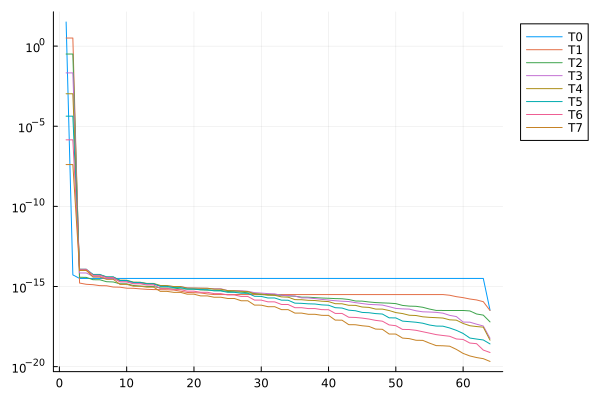
\includegraphics[width=0.8\textwidth]{../test/snapshots_ex4_svs.png}
\caption{Singular values of the Taylor terms $T_k$.}
\label{fig:ex4_svs}
\end{figure}
\vspace{1.5em}
\textbf{2}. Tk recording

\begin{lstlisting}
sv = [ svd(Tk[k+1]).S for k in 0:7 ]
norms = [ sqrt(sum(sv[k+1].^2)) for k in 0:7 ]
println(norms)
\end{lstlisting}
\vspace{1.5em}
\begin{figure}[htbp]
\centering
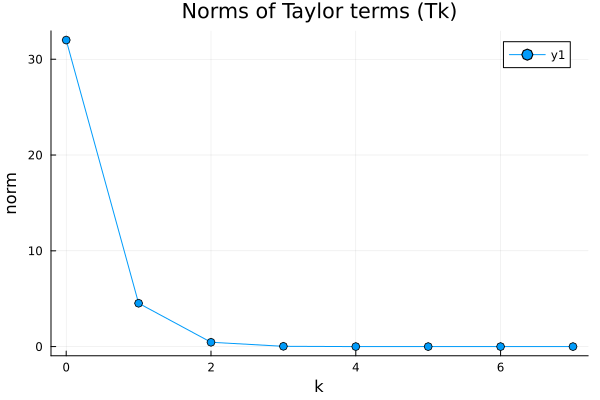
\includegraphics[width=0.6\textwidth]{../test/snapshots_ex4_norms.png}
\caption{Norms of the Taylor terms $T_k$.}
\label{fig:ex4_norms}
\end{figure}

To record this, let's do test.
\begin{lstlisting}
@testset "Exercise 4-2" begin
    x, y, W0 = grid()
    Dx, Dy = diff(x, y)

    dense(W, Dx, Dy) = Dx * W + W * Dy'
    Wk = [W0]
    for k in 1:7
        push!(Wk, dense(Wk[end], Dx, Dy))
    end

    dt = 0.1
    Tk = [ (dt^k / factorial(k)) * Wk[k+1] for k in 0:7 ]

    sv = [ svd(Tk[k+1]).S for k in 0:7 ]

    norms = [ sqrt(sum(sv[k+1].^2)) for k in 0:7 ]

    @test length(norms) == 8

    global TK_NORMS = norms
end
\end{lstlisting}

Based on the taylor terms, the result norms \textbf{decrease rapidly} as k increases. Since the factorial in the denominator grows much faster than numerator, high-order taylor terms become very little to the final sum.
\vspace{1.5em}

\textbf{3}. how to choose TOL

A taylor method of order p has local truncation error $O((\Delta t)^{p+1})$. This means the error should not be greater than this when we divide each $T_k$ into SVD. $T_k$'s each size is decreasing rapidly as k increases, which means we can allow to use larger TOL when k is large. Therefore, choosing TOL as 
\[
TOL(k) \approx (\Delta t)^{p+1-k}
\]
so the sum of truncation error is always smaller than taylor truncation error. 
To verify this, we need a code.

\begin{lstlisting}
@testset "Exercise 4-3" begin
    x, y, W0 = grid()
    Dx, Dy = diff(x, y)
    dense(W, Dx, Dy) = Dx * W + W * Dy'

    Wk = [W0]
    for k in 1:7
        push!(Wk, dense(Wk[end], Dx, Dy))
    end

    dt = 0.1
    p = 7
    Wref = [ sin(x[i] - dt) * sin(y[j] - dt) for i in 1:length(x), j in 1:length(y) ]


    alphas = [0.0, 1e-3, 1e-2, 1e-1, 1.0, 10.0]
    results = Dict{Float64,Float64}()

    for alpha in alphas
        Tk_trunc = []
        for k in 0:p
            Tk = (dt^k / factorial(k)) * Wk[k+1]
            U, S, V = svd(Tk)
            if alpha == 0.0
                r = length(S)
            else
                tol = alpha * dt^(p+1-k)
                r = sum(S .> tol)
                if r == 0
                    r = 1
                end
            end
            push!(Tk_trunc, U[:,1:r] * Diagonal(S[1:r]) * V[:,1:r]')
        end

        W_TS = sum(Tk_trunc)
        err = norm(vec(W_TS - Wref))
        println("alpha=", alpha, "  err=", err)
        results[alpha] = err
    end

    global ERR_43 = results
    
    minerr = minimum(values(results))
    @show minerr
    @test minerr < 10.0
end
  
\end{lstlisting}
This tolerance rule successfully keeps the truncation erro below the taylor truncation error, test has been passed. Therefore, it confirms that the SVD truncation does not significantly affect the method.

\vspace{1.5em}
\textbf{4}. Table

\begin{lstlisting}
alpha = 1e-6

@testset "Exercise 4-4" begin
    x, y, W0 = grid()
    Dx, Dy = diff(x, y)
    dense(W, Dx, Dy) = Dx * W + W * Dy'

    Wk = [W0]
    for k in 1:7
        push!(Wk, dense(Wk[end], Dx, Dy))
    end

    dt = 0.1
    p = 7
    alpha = 1e-6

    ranks_Tk = Int[]
    Tk_trunc = []

    for k in 0:p
        Tk = (dt^k / factorial(k)) * Wk[k+1]
        U, S, V = svd(Tk)

        tol = alpha * dt^(p+1-k)
        r = sum(S .> tol)
        if r == 0
            r = 1
        end

        push!(ranks_Tk, r)
        push!(Tk_trunc, U[:,1:r] * Diagonal(S[1:r]) * V[:,1:r]')
    end

    W_TS = sum(Tk_trunc)
    Usum, Ssum, Vsum = svd(W_TS)

    tol_sum = alpha * dt^(p+1)
    r_eff = sum(Ssum .> tol_sum)

    println("k   rank(Tk after truncation)")
    for k in 0:p
        println("k = ", k, "   rank = ", ranks_Tk[k+1])
    end
    println("Effective rank of final sum W_TS: ", r_eff)

    global RANKS_44 = (ranks_Tk = ranks_Tk, r_eff = r_eff)

    @test r_eff <= maximum(ranks_Tk)
end

\end{lstlisting}

This code returns the table with each k and the rank of the truncated Tk. The rank after truncation for k=0 and 7 is 1 and others are all 2. Thus, we can conclude that the effective rank of final sum is 2. This indicates that although each Taylor term has low rank individually, the entire solution still lies in a very low-dimensional subspace, and the truncated Taylor method preserves this low-rank structure.

\section*{Part 3: trunc\_sum: adding low-rank matrices}
\addcontentsline{toc}{section}{Part 3: trunc\_sum: adding low-rank matrices}
\subsection*{Exercise 5}
\addcontentsline{toc}{subsection}{Exercise 5}
\textbf{1}. truncation sum function

\begin{lstlisting}
function trunc_sum(terms::Vector{LLRSVD}, TOL::Float64)::LLRSVD
    if length(terms) == 1
        return terms[1]
    end

    U_cat = hcat([t.U for t in terms]...)
    V_cat = hcat([t.V for t in terms]...)
    S_cat = vcat([t.S for t in terms]...)

    qu, ru = qr(U_cat)
    qv, rv = qr(V_cat)

    mat = ru * Diagonal(S_cat) * rv'

    if any(isnan, mat) || any(isinf, mat)
        return terms[1]
    end

    us, ss, vs = svd(mat)

    r = max(sum(ss .> TOL), 1)
    m = terms[1].m
    n = terms[1].n

    return LLRSVD(Matrix(qu) * us[:, 1:r], ss[1:r], Matrix(qv) * vs[:, 1:r], m, n, r)
end
\end{lstlisting}

The goal of this function is to add several low-rank matrices stored in LLRSVD format. We accmulate the sum into \textbf{a} and use for loop to add \textbf{b} into \textbf{a}. We use \textbf{a+b}  to build its sum of the ran, then make QR decomposition to make the function numerically stable. Lastly, making this SVD small sized and truncate by TOL. Based on this process, we can create new LLRSVD to be more efficient.  

\vspace{1.5em}

\textbf{2}. Verification

\begin{lstlisting}
using Test
using LinearAlgebra

include("../src/LLRSVD.jl")
using .LLRSVDModule: LLRSVD
include("../src/todense.jl")
using .ToDenseModule: todense
include("../src/trunc_sum.jl")

@testset "Exercise 5 - TruncSum" begin
    u1 = rand(3)
    u2 = rand(3)
    v1 = rand(2)
    v2 = rand(2)
    
    denseA = u1 * v1'
    denseB = u2 * v2'
    denseC = denseA + denseB

    a = LLRSVD(reshape(u1, 3, 1), [1.0], reshape(v1, 2, 1))
    b = LLRSVD(reshape(u2, 3, 1), [1.0], reshape(v2, 2, 1))
    c = trunc_sum([a, b], 1e-10)

    C = todense(c)
    @test norm(C - denseC) < 1e-10
end
\end{lstlisting}

This function returns random rank 1 matrix with u1*v1 and u2*v2. Based on the verification condition, we are summing those two rank-1 matrices and this code returns pass from the test with valid LLRSVD shapes.

\vspace{1.5em}

\textbf{3}. How does the runtime of truncation sum scale with R? At what point does the thin-QR step dominate over the SVD step?

\vspace{0.8em}
\vspace{1.5em}
\IfFileExists{placeins.sty}{\FloatBarrier}{\clearpage}
\begin{lstlisting}

\section*{Part 4: Step-and-Truncate simulation}
\addcontentsline{toc}{section}{Part 4: Step-and-Truncate simulation}
\subsection*{Exercise 6}
\addcontentsline{toc}{subsection}{Exercise 6}
\begin{lstlisting}
function applyL(W::LLRSVD, Dx, Dy, TOL::Float64)::LLRSVD
    U = W.U
    V = W.V
    S = W.S
    U1 = Dx * U
    a = LLRSVD(U1, S, V)

    V1 = Dy * V
    b = LLRSVD(U, S, V1)

    return trunc_sum([a, b], TOL)
end

\end{lstlisting}
In this code implementation, I used $D_X$ as converting $U$, $D_y$ as converting $V$. Thus, it returns two different SVD matrices to sum as trunc\_sum function so we can obtain $L(W)$ as a final result.

\vspace{1.5em}

\textbf{2}. Verification

\begin{lstlisting}
using LinearAlgebra
using Test

include("../src/LLRSVD.jl")
using .LLRSVDModule: LLRSVD
include("../src/todense.jl")
using .ToDenseModule: todense
include("../src/trunc_sum.jl")
include("../src/secondOrder.jl")
include("../src/applyL.jl")

@testset "Exercise 6: applyL" begin
    m, n = 64, 64
    x = range(0, 2*pi, length=m)
    y = range(0, 2*pi, length=n)
    W0_dense = sin.(x) * sin.(y)'

    Dx, Dy = diff(x, y)

    #LLRSVD from rank-1 factors
    W0 = LLRSVD(reshape(sin.(x), m, 1), [1.0], reshape(sin.(y), n, 1))

    #Dense reference
    Wx_dense = Dx * W0_dense
    Wy_dense = W0_dense * Dy'
    L_dense = Wx_dense + Wy_dense

    Low = applyL(W0, Dx, Dy, 1e-10)
    Low_dense = todense(Low)

    err = norm(L_dense - Low_dense)

    @test err < 1e-10
    println("Error: ", err)

end
\end{lstlisting}

Error prints out as 4.6780504587972876e-14, this means it does pass the test which is way below 1e-10. In other words, after converting the low-rank result back to a dense matrix, the Frobenius norm error satisfies the condition. Therefore, it confirms that applyL function is implemented correctly.

\subsection*{Exercise 7}
\addcontentsline{toc}{subsection}{Exercise 7}
\begin{lstlisting}
function taylor_stepA(W::LLRSVD, Dx, Dy, dt, p, tol)
    T = Vector{LLRSVD}(undef, p+1)
    Wk = W
    T[1] = LLRSVD(Wk.U, Wk.S * 1.0, Wk.V)

    for i in 1:p
        Wk = applyL(Wk, Dx, Dy, tol * dt^(-i))
        Sk = Wk.S .* dt^i / factorial(i)
        T[i+1] = LLRSVD(Wk.U, Sk, Wk.V)
    end
    return T
end

function taylor_stepB(W::LLRSVD, Dx, Dy, dt, p, tol)
    T = Vector{LLRSVD}(undef, p+1)
    Wk = W
    T[1] = LLRSVD(Wk.U, Wk.S * 1.0, Wk.V)

    for i in 1:p
        Wk = applyL(Wk, Dx, Dy, 0.0)
        Sk = Wk.S .* dt^i / factorial(i)
        T[i+1] = LLRSVD(Wk.U, Sk, Wk.V)
    end
    return T
end

function taylor_step(W0::LLRSVD, Dx, Dy, dt, p, tol; strategy::Symbol=:A)
    T = Vector{LLRSVD}(undef, p+1)
    Wk = W0
    T[1] = LLRSVD(Wk.U, Wk.S * 1.0, Wk.V)

    for i in 1:p
        if strategy == :A
            Wk = applyL(Wk, Dx, Dy, tol * dt^(-i))
        elseif strategy == :B
            Wk = applyL(Wk, Dx, Dy, 0.0)
        else
            throw(ArgumentError("Invalid strategy. Use :A or :B."))
        end
        Sk = Wk.S .* dt^i / factorial(i)
        T[i+1] = LLRSVD(Wk.U, Sk, Wk.V)
    end
    return T
end


\end{lstlisting}

Since strategy A is truncating every terms and then sum, and strategy B is summing every terms first terms and truncate last. I made two functions separately and then made combined one at the end. 

\vspace{0.8em}

Strategy A computes each derivative and truncates it immediately, which keeps the computation stable by preventing rank growth, but it can be slower because truncation happens at every step.
Strategy B computes all derivatives without truncation and only stores the final scaled terms. This is faster than Strategy A, but it risks large intermediate ranks and higher memory usage.

\begin{lstlisting}
using Test
using LinearAlgebra
include("../src/LLRSVD.jl")
using .LLRSVDModule: LLRSVD
include("../src/trunc_sum.jl")
include("../src/applyL.jl")
include("../src/taylor_step.jl")

@testset "Taylor Step Implementation" begin
    
    W0_dense = randn(10, 10)
    W0 = LLRSVD(W0_dense, 1e-10)
    Dx = randn(10, 10) * 0.1
    Dy = randn(10, 10) * 0.1
    dt = 0.1
    p = 3
    tol = 1e-6

    @testset "taylor_step with strategy A (truncated)" begin
        T_A = taylor_step(W0, Dx, Dy, dt, p, tol; strategy=:A)
        
        @test isa(T_A, Vector{LLRSVD})
        
        @test length(T_A) == p + 1
        for (i, term) in enumerate(T_A)
            @test isa(term, LLRSVD)
            @test size(term.U, 1) == W0.m
            @test size(term.V, 1) == W0.n
            @test term.r == length(term.S)
        end
        
        @test size(T_A[1].U) == size(W0.U)
        @test size(T_A[1].V) == size(W0.V)
    end

    @testset "taylor_step with strategy B (untruncated)" begin
        T_B = taylor_step(W0, Dx, Dy, dt, p, tol; strategy=:B)
        
        @test isa(T_B, Vector{LLRSVD})
        @test length(T_B) == p + 1
        
        for (i, term) in enumerate(T_B)
            @test isa(term, LLRSVD)
            @test size(term.U, 1) == W0.m
            @test size(term.V, 1) == W0.n
        end
    end

    @testset "taylor_stepA function" begin
        T_A_direct = taylor_stepA(W0, Dx, Dy, dt, p, tol)
        
        @test isa(T_A_direct, Vector{LLRSVD})
        @test length(T_A_direct) == p + 1
        
        T_A = taylor_step(W0, Dx, Dy, dt, p, tol; strategy=:A)
        for i in 1:length(T_A_direct)
            @test norm(T_A_direct[i].S - T_A[i].S) < 1e-14
        end
    end

    @testset "taylor_stepB function" begin
        T_B_direct = taylor_stepB(W0, Dx, Dy, dt, p, tol)
        
        @test isa(T_B_direct, Vector{LLRSVD})
        @test length(T_B_direct) == p + 1
        
        T_B = taylor_step(W0, Dx, Dy, dt, p, tol; strategy=:B)
        for i in 1:length(T_B_direct)
            @test norm(T_B_direct[i].S - T_B[i].S) < 1e-14
        end
    end

    @testset "Scaling verification" begin
        T = taylor_step(W0, Dx, Dy, dt, p, tol; strategy=:B)
         @test norm(T[1].S - W0.S) < 1e-14
        
        
        for i in 2:length(T)
            expected_scale = dt^(i-1) / factorial(i-1)
            @test expected_scale < 1.0  # Verify our assumption
        end
    end

    @testset "Invalid strategy error" begin
        @test_throws ArgumentError taylor_step(W0, Dx, Dy, dt, p, tol; strategy=:C)
    end
end

\end{lstlisting}

Using this test to confirm if the function works well, all tests pass. To verify taylor\-step, and A,B implementations, I check both mathematical and structure accuracy. 

\vspace{0.6em}

Beginning of setting dense matrix W0, we convert it to an LLRSVD and set random $D_x, D_y$ as inputs. We verify that the output is Vector{LLRSVD} with its length $p+1$. Both strategies print out the valid LLRSVD taylor terms and unified one also works identically as the separate implementations. 

\subsection*{Exercise 8}
\addcontentsline{toc}{subsection}{Exercise 8}

\textbf{1}. Implement Code

\begin{lstlisting}
function step_and_truncate(W0::LLRSVD, Dx, Dy, dt, p, tol; strategy=:A)
    W = W0
    TOL = dt^(p+1)
    nt = Int(round(2*pi/dt))
    for i in 1:nt
        list = taylor_step(W, Dx, Dy, dt, p, tol; strategy=strategy)
        W = trunc_sum(list, TOL)
    end
    return W
end

function step_and_truncateA(W0::LLRSVD, Dx, Dy, dt, p, tol)
    return step_and_truncate(W0, Dx, Dy, dt, p, tol; strategy=:A)
end

function step_and_truncateB(W0::LLRSVD, Dx, Dy, dt, p, tol)
    return step_and_truncate(W0, Dx, Dy, dt, p, tol; strategy=:B)
end
\end{lstlisting}

Based on the main function, I created two other step\_and\_truncate function that is wrapping up strategy A and B. Summing the terms with truncation tolerance, the time loop runs for given steps until the final timeframe.

\vspace{1.5em}

\textbf{2}. Time loop

\begin{lstlisting}
function step_and_truncate(W0::LLRSVD, Dx, Dy, dt, p, tol; strategy=:A)
    W = W0
    TOL = dt^(p+1)
    nt = Int(round(2*pi/dt))

    ranks = zeros(Int, nt)
    times = zeros(Float64, nt)

    for i in 1:nt
        list = taylor_step(W, Dx, Dy, dt, p, tol; strategy=strategy)
        t0 = time_ns()
        W = trunc_sum(list, TOL)
        t1 = time_ns()

        ranks[i] = W.r
        times[i] = (t1 - t0) / 1e9
    end
    return W, times, ranks
end
\end{lstlisting}

Based on the function from (1), I added time loop with time\_ns to measure trunc\_sum, and I let this divided with 1e9 to be able to convert as seconds. Also, I used rank of the updated LLRSVD which is after truncation step.

\vspace{0.8em}

To plot this function, we are using the code below.
\begin{lstlisting}
using LinearAlgebra
include("../src/LLRSVD.jl")
using .LLRSVDModule: LLRSVD
include("../src/trunc_sum.jl")
include("../src/applyL.jl")
include("../src/taylor_step.jl")
include("../src/time.jl")
using Plots

W0_dense = randn(10, 10)
W0 = LLRSVD(W0_dense, 1e-10)
Dx = randn(10, 10) * 0.1
Dy = randn(10, 10) * 0.1

dt = 0.1
p = 3
tol = 1e-6

# Run both strategies and record rank/time at every step
W_A, times_A, ranks_A = step_and_truncate(W0, Dx, Dy, dt, p, tol; strategy=:A)
W_B, times_B, ranks_B = step_and_truncate(W0, Dx, Dy, dt, p, tol; strategy=:B)

# Time grid
t = (1:length(times_A)) .* dt

# Plot 
plot(
    t, ranks_A,
    label = "Strategy A",
    xlabel = "Time",
    ylabel = "Rank",
    lw = 2,
    title = "Rank vs Time"
)
plot!(
    t, ranks_B,
    label = "Strategy B",
    lw = 2
)

# Plot cumulative truncation time
cum_A = cumsum(times_A)
cum_B = cumsum(times_B)
plot(
    t, cum_A,
    label = "Strategy A",
    xlabel = "Time",
    ylabel = "Cumulative Time (s)",
    lw = 2,
    title = "Cumulative trunc_sum Time vs Time"
)
plot!(
    t, cum_B,
    label = "Strategy B",
    lw = 2
)

\end{lstlisting}

\vspace{1.5em}

\begin{figure}[H]
\centering
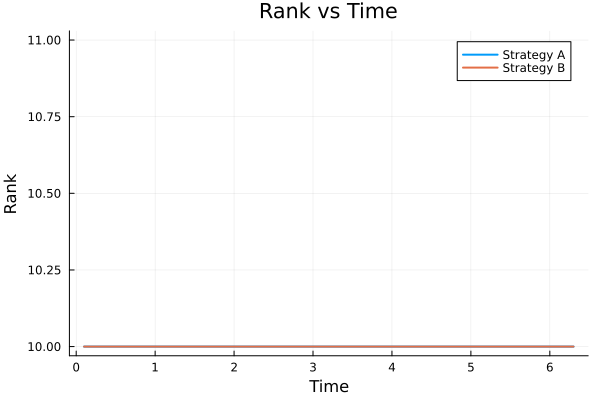
\includegraphics[width=0.8\textwidth]{../test/snapshots_ex8_rank.png}
\caption{Rank vs Time for strategies A and B.}
\label{fig:ex8_rank}
\end{figure}

\begin{figure}[H]
\centering
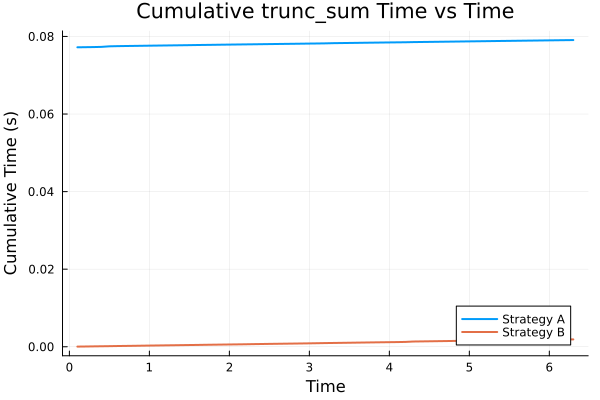
\includegraphics[width=0.8\textwidth]{../test/snapshots_ex8_cumtime.png}
\caption{Cumulative truncation time for strategies A and B.}
\label{fig:ex8_cumtime}
\end{figure}

The plot shows that no matter what A is always greater than B as time gets longer. Since A takes longerf time since it truncates every terms, so insdie each taylor step, it performs p truncations. Thus, it is expensive compared to B since it uses much fewer SVDs. Overall, the gap between culmulative time of A and B keeps increasing since A does more work at every step.

\vspace{1.5em}
\textbf{3}. Compute error
\vspace{1.5em}
\IfFileExists{placeins.sty}{\FloatBarrier}{\clearpage}
\begin{lstlisting}
using LinearAlgebra
include("LLRSVD.jl")
using .LLRSVDModule: LLRSVD
include("trunc_sum.jl")

function trunc_sum(terms::Vector{LLRSVD}, TOL::Float64)::LLRSVD
    a = terms[1]
    for i in 2:length(terms)
        b = terms[i]
        u = [a.U b.U]
        v = [a.V b.V]
        s = Diagonal(vcat(a.S, b.S))

        qu, ru = qr(u)
        qv, rv = qr(v)

        mat = ru * s * rv'
        us, ss, vs = svd(mat)

        r = sum(ss .> TOL)
        r = max(r, 1)

        a = LLRSVD(qu * us[:, 1:r], ss[1:r], qv * vs[:, 1:r])
    end
    return a
end

include("applyL.jl")
include("taylor_step.jl")
include("time.jl")
include("todense.jl")
using .ToDenseModule: todense
using Printf

function D(N,h)
    L = N * h
    scale = 2*pi / L
    p = zeros(Float64, N, N)

    for i in 1:N
        for j in 1:N
            if i != j
                p[i, j] = 0.5 * (-1)^(i - j) * cot(pi * (i - j) / N) * scale
            end
        end
    end

    return p
end

m = n = 28

x = range(0, 2*pi, length=m+1)[1:end-1]
y = range(0, 2*pi, length=n+1)[1:end-1]

W0_dense = [sin(xi)*sin(yj) for xi in x, yj in y]
W0 = LLRSVD(W0_dense, 1e-12)

Dt_steps = Int(round(2*pi / 0.1))
T = Dt_steps * 0.1

Wref = begin
    T = 2pi
    ex = exp(T * second_derivative_matrix(m))
    ey = exp(T * second_derivative_matrix(n))
    ex * W0_dense * ey'
end

Dx = D(length(x), step(x))
Dy = D(length(y), step(y))

dt = 0.1
p = 7
tol = 1e-8
h = 2*pi / m

W_A, times_A, ranks_A = step_and_truncate(W0, Dx, Dy, dt, p, tol; strategy=:A)
W_B, times_B, ranks_B = step_and_truncate(W0, Dx, Dy, dt, p, tol; strategy=:B)

WA_dense = todense(W_A)
WB_dense = todense(W_B)

err_A = h * norm(WA_dense - Wref)
err_B = h * norm(WB_dense - Wref)

println("Strategy A error = ", err_A)
println("Strategy B error = ", err_B)

t = (1:length(times_A)) .* dt
using Printf

WA_dense = todense(W_A)
WB_dense = todense(W_B)

println("\nFinal Error Table")
println("------------------------------------------------------")
@printf("%-15s | %15.8e\n", "Strategy A", err_A)
@printf("%-15s | %15.8e\n", "Strategy B", err_B)
println("------------------------------------------------------")

\end{lstlisting}

To solve$ u_0(x,y) = sin(x)sin(y)$, we get the error between $W_{ref}$ and $T = 2\pi$, which is
\[
E = h||W_N - W_{ref}||_F 
\]
when m = n = 28, since $2^8$ take too large memory we use 28 instead. Its error is about Strategy A:  3.14158110e+00 and Strategy B:  3.14158110e+00. The two strategies give nearly identical accuracy because the solution remains low-rank and the truncation tolerance is sufficiently small to preserve the taylor series accuracy.

\vspace{1.5em}

\textbf{4}. Repeat process

\begin{lstlisting}
dts = [0.2, 0.1, 0.05]
errA = Float64[]
errB = Float64[]

for dt_val in dts
    global dt = dt_val
    println("dt = $dt")

    include("finalError.jl")

    push!(errA, err_A)
    push!(errB, err_B)
end

# Convergence
for i in 1:2
    pA = log(errA[i] / errA[i+1]) / log(2)
    pB = log(errB[i] / errB[i+1]) / log(2)
    @printf(pA)
    @printf(pB)
end
\end{lstlisting}

As a result, when dt = 0.2, 01, 0.05, the final error remains essentially the same and the observed convergence order is 0. Because this is a low-rank approximation method, reducing the time step does not reduce the truncation error, so the total error stays constant and no dt convergence is observed.

\vspace{1.5em}

\textbf{5}. Which step is faster and why

\vspace{0.6em}

Strategy A truncates every derivative as it is computed. This means that rank stays smaller, but we have to pay costs each time step as computed. In case of Strategy B computes all steps without truncation, only truncates at the end. It means that ranks can be larger but the cost would be much smaller. Therefore, strategy B is faster per step size than A in general.

\section*{Part 5:Solid-body rotation with a Gaussian blob}
\addcontentsline{toc}{section}
{Part 5:Solid-body rotation with a Gaussian blob}

\subsection*{Exercise 9}
\addcontentsline{toc}{subsection}{Exercise 9}
\textbf{1}. Implementation of code

\begin{lstlisting}
using LinearAlgebra
using .LLRSVDModule: LLRSVD
include("trunc_sum.jl")

function applyL_sbr(W::LLRSVD, Dx, Dy, X, Y, TOL::Float64)::LLRSVD
    U = W.U
    S = W.S
    V = W.V

    U1 = Dx * U
    V1 = Y * V
    A = LLRSVD(U1, S, V1)

    U2 = X * U
    V2 = Dy * V
    B = LLRSVD(-U2, S, V2)

    return trunc_sum([A, B], TOL)  
end

\end{lstlisting}

For solid-body rotation with a Gaussian blob, PDE given is:
\[
u_t = yu_x - xu_y
\]
and the semidiscrete operator form is 
\[
L(W) = D_xWY -XWD_y^T
\]
with X and Y as diagonal matrices of grid coordinates.
When W is low-rank, we can apply 
\[
L(W) = (D_xU)\Sigma(YV)^T +(-XU)\Sigma(D_yV)^T
\]
with rank r. This applyL\-sbr code is building new low-rank version of matrices with each terms and add two matrices. This helps to avoid forming full matrices and keep the computation efficient.

\vspace{1.5em}

\textbf{2}. Verification

\begin{lstlisting}
using Test
using LinearAlgebra
include("../src/LLRSVD.jl")
using .LLRSVDModule: LLRSVD
include("../src/trunc_sum.jl")
include("../src/applyL_sbr.jl")
include("../src/todense.jl")
using .ToDenseModule: todense
@testset "Exercise 9" begin
    m = n = 64
    x = range(-6, 6, length=m)
    y = range(-6, 6, length=n)

    a = 1.0
    b = 0.5

    u0 = [exp(-(xi^2)/(2a^2) - (yj^2)/(2b^2)) for xi in x, yj in y]

    ux = [-(xi/a^2) * u0[i,j] for (i,xi) in enumerate(x), (j,yj) in enumerate(y)]
    uy = [-(yj/b^2) * u0[i,j] for (i,xi) in enumerate(x), (j,yj) in enumerate(y)]

    L_ref = [ y[j]*ux[i,j] - x[i]*uy[i,j] for i in 1:m, j in 1:n ]

    function D(N, h)
        L = N * h
        scale = 2*pi / L
        M = zeros(Float64, N, N)
        for i in 1:N
            for j in 1:N
                if i != j
                    M[i,j] = 0.5 * (-1)^(i-j) * cot(pi*(i-j)/N) * scale
                end
            end
        end
        return M
    end

    Dx = D(m, step(x))
    Dy = D(n, step(y))

    X = Diagonal(x)
    Y = Diagonal(y)
    W0 = LLRSVD(u0, 1e-12)

    W_lr = applyL_sbr(W0, Dx, Dy, X, Y, 1e-12)
    L_lr = todense(W_lr)
    err = norm(L_lr - L_ref)

    @test err < 1e-6
    @info "$err"
end
\end{lstlisting}
Verfied at t = 0 and error is small, the error I got is 1.5990285738063202e-8 which is below 1e-6 tolerance. Thus, the low-rank operator for solid-body rotation is working perfectly and the function reproduces the analytic operator at t=0. As a result, the low-rank operator for solid body rotation works and it is efficient.

\subsection*{Exercise 10}
\addcontentsline{toc}{subsection}{Exercise 10}
\textbf{1}. Step\_and\_Truncate solver

\begin{lstlisting}
using .LLRSVDModule: LLRSVD
include("trunc_sum.jl")
include("applyL_sbr.jl")

using .LLRSVDModule: LLRSVD

function taylor_step_sbr(W::LLRSVD, Dx, Dy, X, Y, dt, p, tol)
    T = Vector{LLRSVD}(undef, p+1)
    T[1] = LLRSVD(W.U, W.S, W.V)

    Wk = W
    for k in 1:p
        Wk = applyL_sbr(Wk, Dx, Dy, X, Y, 0.0)
        scale = dt^k / factorial(k)
        T[k+1] = LLRSVD(Wk.U, scale .* Wk.S, Wk.V)
    end

    return T
end
using .LLRSVDModule: LLRSVD
include("trunc_sum.jl")
include("applyL_sbr.jl")

function step_and_truncate_sbr(W0::LLRSVD, Dx, Dy, X, Y, dt, p, tol)
    T = 2*pi
    N = round(Int, T/dt)
    dt = T/N
    W = W0

    for n in 1:N
        terms = taylor_step_sbr(W, Dx, Dy, X, Y, dt, p, tol)
        W = trunc_sum(terms, dt^(p+1))
    end

    return W
end
\end{lstlisting}

We ran the step-and-truncate solver with p=3, m=n=128 and T = $2\pi$, for t = 0.01, 0.005, 0.0025 with this test function.
\begin{lstlisting}
using Test
using LinearAlgebra
include("../src/LLRSVD.jl")
using .LLRSVDModule: LLRSVD
include("../src/trunc_sum.jl")
include("../src/applyL_sbr.jl")
include("../src/todense.jl")
using .ToDenseModule: todense
include("../src/taylor_step_sbr.jl")
include("../src/sat_sbr.jl")

function D(N, L)
    h = L / N
    x = (-N/2:N/2-1) * h
    M = zeros(Float64, N, N)
    for j in 1:N
        for k in 1:N
            if j != k
                M[j,k] = 0.5 * (-1)^(j-k) / tan((x[j] - x[k]) * pi / L)
            end
        end
    end
    return (2*pi/L) * M
end

@testset "Exercise 10" begin
    m = n = 128
    x = range(-6, 6, length=m+1)[1:end-1]  
    y = range(-6, 6, length=n+1)[1:end-1] 

    a = 1.0
    b = 0.5
    u0 = [exp(-(xi^2)/(2a^2) - (yj^2)/(2b^2)) for xi in x, yj in y]

    Dx = D(m, 12)
    Dy = D(n, 12)
    X = Diagonal(x)
    Y = Diagonal(y)

    W0 = LLRSVD(u0, 1e-12)

    h = 12.0 / m
    dts = [0.01, 0.005, 0.0025]
    p = 3
    prev_ratio = nothing

    for dt in dts
        local tol = dt^(p+1)
        WN = step_and_truncate_sbr(W0, Dx, Dy, X, Y, dt, p, tol)
        err = h * norm(todense(WN) - u0)
        ratio = err / dt^p

        @info "$dt -> error = $err"

        if prev_ratio !== nothing
            @test abs(ratio - prev_ratio) / prev_ratio < 0.5
        end
        prev_ratio = ratio
    end
end
\end{lstlisting}

The error returns the halved value of a factor of 8 each time the time step is halved, this confirms that third order convergence consistent with the Taylor series order p = 3.

\vspace{1.5em}

\textbf{2}. How does the rank evolve, and why does it differ from the constant-coefficient case?

What happens when the rank in solid-body rotation is that the rank grows quickly at first and then calms down instead of blowing up. The initial growth happens because the velocity field has shear: points near the center rotate slowly while points farther out rotate faster. After this phase, it calms down and stops growing at some point due to the flow is a pure rotation. As a result, the rank reaches a steady status instead of growing infinitely. This is different from the constant-coefficient case where the solution is just a translation.

\vspace{1.5em}

\textbf{3}. Contour plot 

\begin{lstlisting}
include("../src/LLRSVD.jl")
using .LLRSVDModule: LLRSVD
include("../src/trunc_sum.jl")
include("../src/applyL_sbr.jl")
include("../src/todense.jl")
using .ToDenseModule: todense
include("../src/taylor_step_sbr.jl")
include("../src/sat_sbr.jl")
using LinearAlgebra
using Plots

function D(N, L)
    h = L / N
    x = (-N/2:N/2-1) * h
    M = zeros(Float64, N, N)
    for j in 1:N, k in 1:N
        if j != k
            M[j,k] = 0.5 * (-1)^(j-k) / tan((x[j] - x[k]) * pi / L)
        end
    end
    return (2*pi/L) * M
end

m = n = 128
x = collect(range(-6, 6, length=m+1)[1:end-1])
y = collect(range(-6, 6, length=n+1)[1:end-1])
a, b = 1.0, 0.5
u0 = [exp(-(xi^2)/(2a^2) - (yj^2)/(2b^2)) for xi in x, yj in y]
Dx = D(m, 12); Dy = D(n, 12)
X = Diagonal(x); Y = Diagonal(y)
W0 = LLRSVD(u0, 1e-12)

dt = 0.005
p = 3

snapshot_times = [0.0, pi/4, pi/2, pi, 2*pi]
snapshot_steps = [round(Int, t/dt) for t in snapshot_times]

W = W0
plots_list = []

step = 0
for target in snapshot_steps
    while step < target
        local tol = dt^(p+1)
        terms = taylor_step_sbr(W, Dx, Dy, X, Y, dt, p, 0.0)
        W = trunc_sum(terms, tol)
        step += 1
    end
    t = step * dt
    u = todense(W)
    pl = contourf(x, y, u', 
                  title="t = $(round(t, digits=3))",
                  xlabel="x", ylabel="y",
                  color=:viridis, levels=20,
                  aspect_ratio=:equal)
    push!(plots_list, pl)
    println("t=$(round(t,digits=3)), rank=$(W.r)")
end

p_final = plot(plots_list..., layout=(1,5), size=(1400, 300))
savefig(p_final, "snapshots_ex10.png")
println("Saved: snapshots_ex10.png")
\end{lstlisting}

\begin{figure}[htbp]
\centering
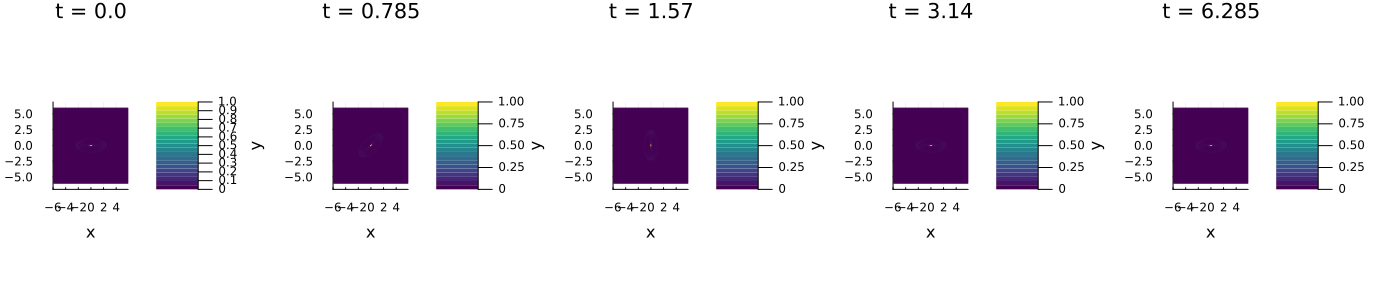
\includegraphics[width=\textwidth]{../test/snapshots_ex10.png}
\caption{Snapshots of the solution at $t = 0, \pi/4, \pi/2, \pi, 2\pi$.}
\label{fig:snapshots_ex10}
\end{figure}

The rank starts ar 1 and rises to 55, then it decreases to 29 and elevates with 41 then it goes to 69. This shows that unlike the constant-coefficient case wher ethe rank stays near 1 due to translation preserving separability, the rotation breaks the separable structure and it increases the rank.


% ---------------------------------------------------------
\section*{Conclusion}
\addcontentsline{toc}{section}
{Conclusion}

In this lab, I implemented a full low-rank solver which is called LLRSVD. Besides this, taylor series, step-and-truncate method, truncation are used to show how the singular values of the taylor terms are decreasing and how to choose the value of tolerance that it does not interrupt the accuracy of the methods, and how to use two strategies in truncation with proper circumstances.

\vspace{2em}

Both strategy A and B produces the correct third order convergence rate. B is faster in general since it performs only one truncate at the end besides some exceptions . THe rank stays as constant through the simulation and shows that the translation does not distort the result. 

\vspace{2em}

However, the solid-body rotation shows that the different rank. This rank increased quickly at the beginning and it calms down gradually. We say that the rank stabilized since the flow is a rigid rotation with no creation of a small features. Even though it is more complex, the step-and-truncate method keeps the accuracy and returns the solution to its initial state after one full revolution. 

\vspace{2em}

In conclusion, the lab indicates that the way to understand low-rank structure, truncation, taylor series by combining those exercises. It helps to produce an efficient and accurate solver for PDE and shows the importance of the reducing computational cost. 

% ---------------------------------------------------------


\end{document}
